\chapter{Dữ liệu và phương pháp nghiên cứu}
\label{ch:phuong-phap}

Chương này trình bày chi tiết kiến trúc hệ thống, quy trình xử lý dữ liệu và thiết kế các mô hình học máy trong khung thực nghiệm \textbf{DepSev-ML}. Để trả lời các câu hỏi nghiên cứu, phương pháp luận được xây dựng dựa trên nguyên tắc module hóa, kiểm soát chặt chẽ quy trình tiền xử lý nhằm tránh rò rỉ dữ liệu, và thử nghiệm các kiến trúc phân loại từ phẳng, phân cấp đến thứ bậc.

\section{Tổng quan quy trình nghiên cứu DepSev-ML}
\label{sec:kien-truc-tong-the}

Quy trình thực nghiệm DepSev-ML được tổ chức thành 7 bước chính như mô tả trong Hình \ref{fig:overall-architecture}.

\begin{figure}[htbp]{Sơ đồ quy trình nghiên cứu thực nghiệm 7 bước của DepSev-ML}
\centering
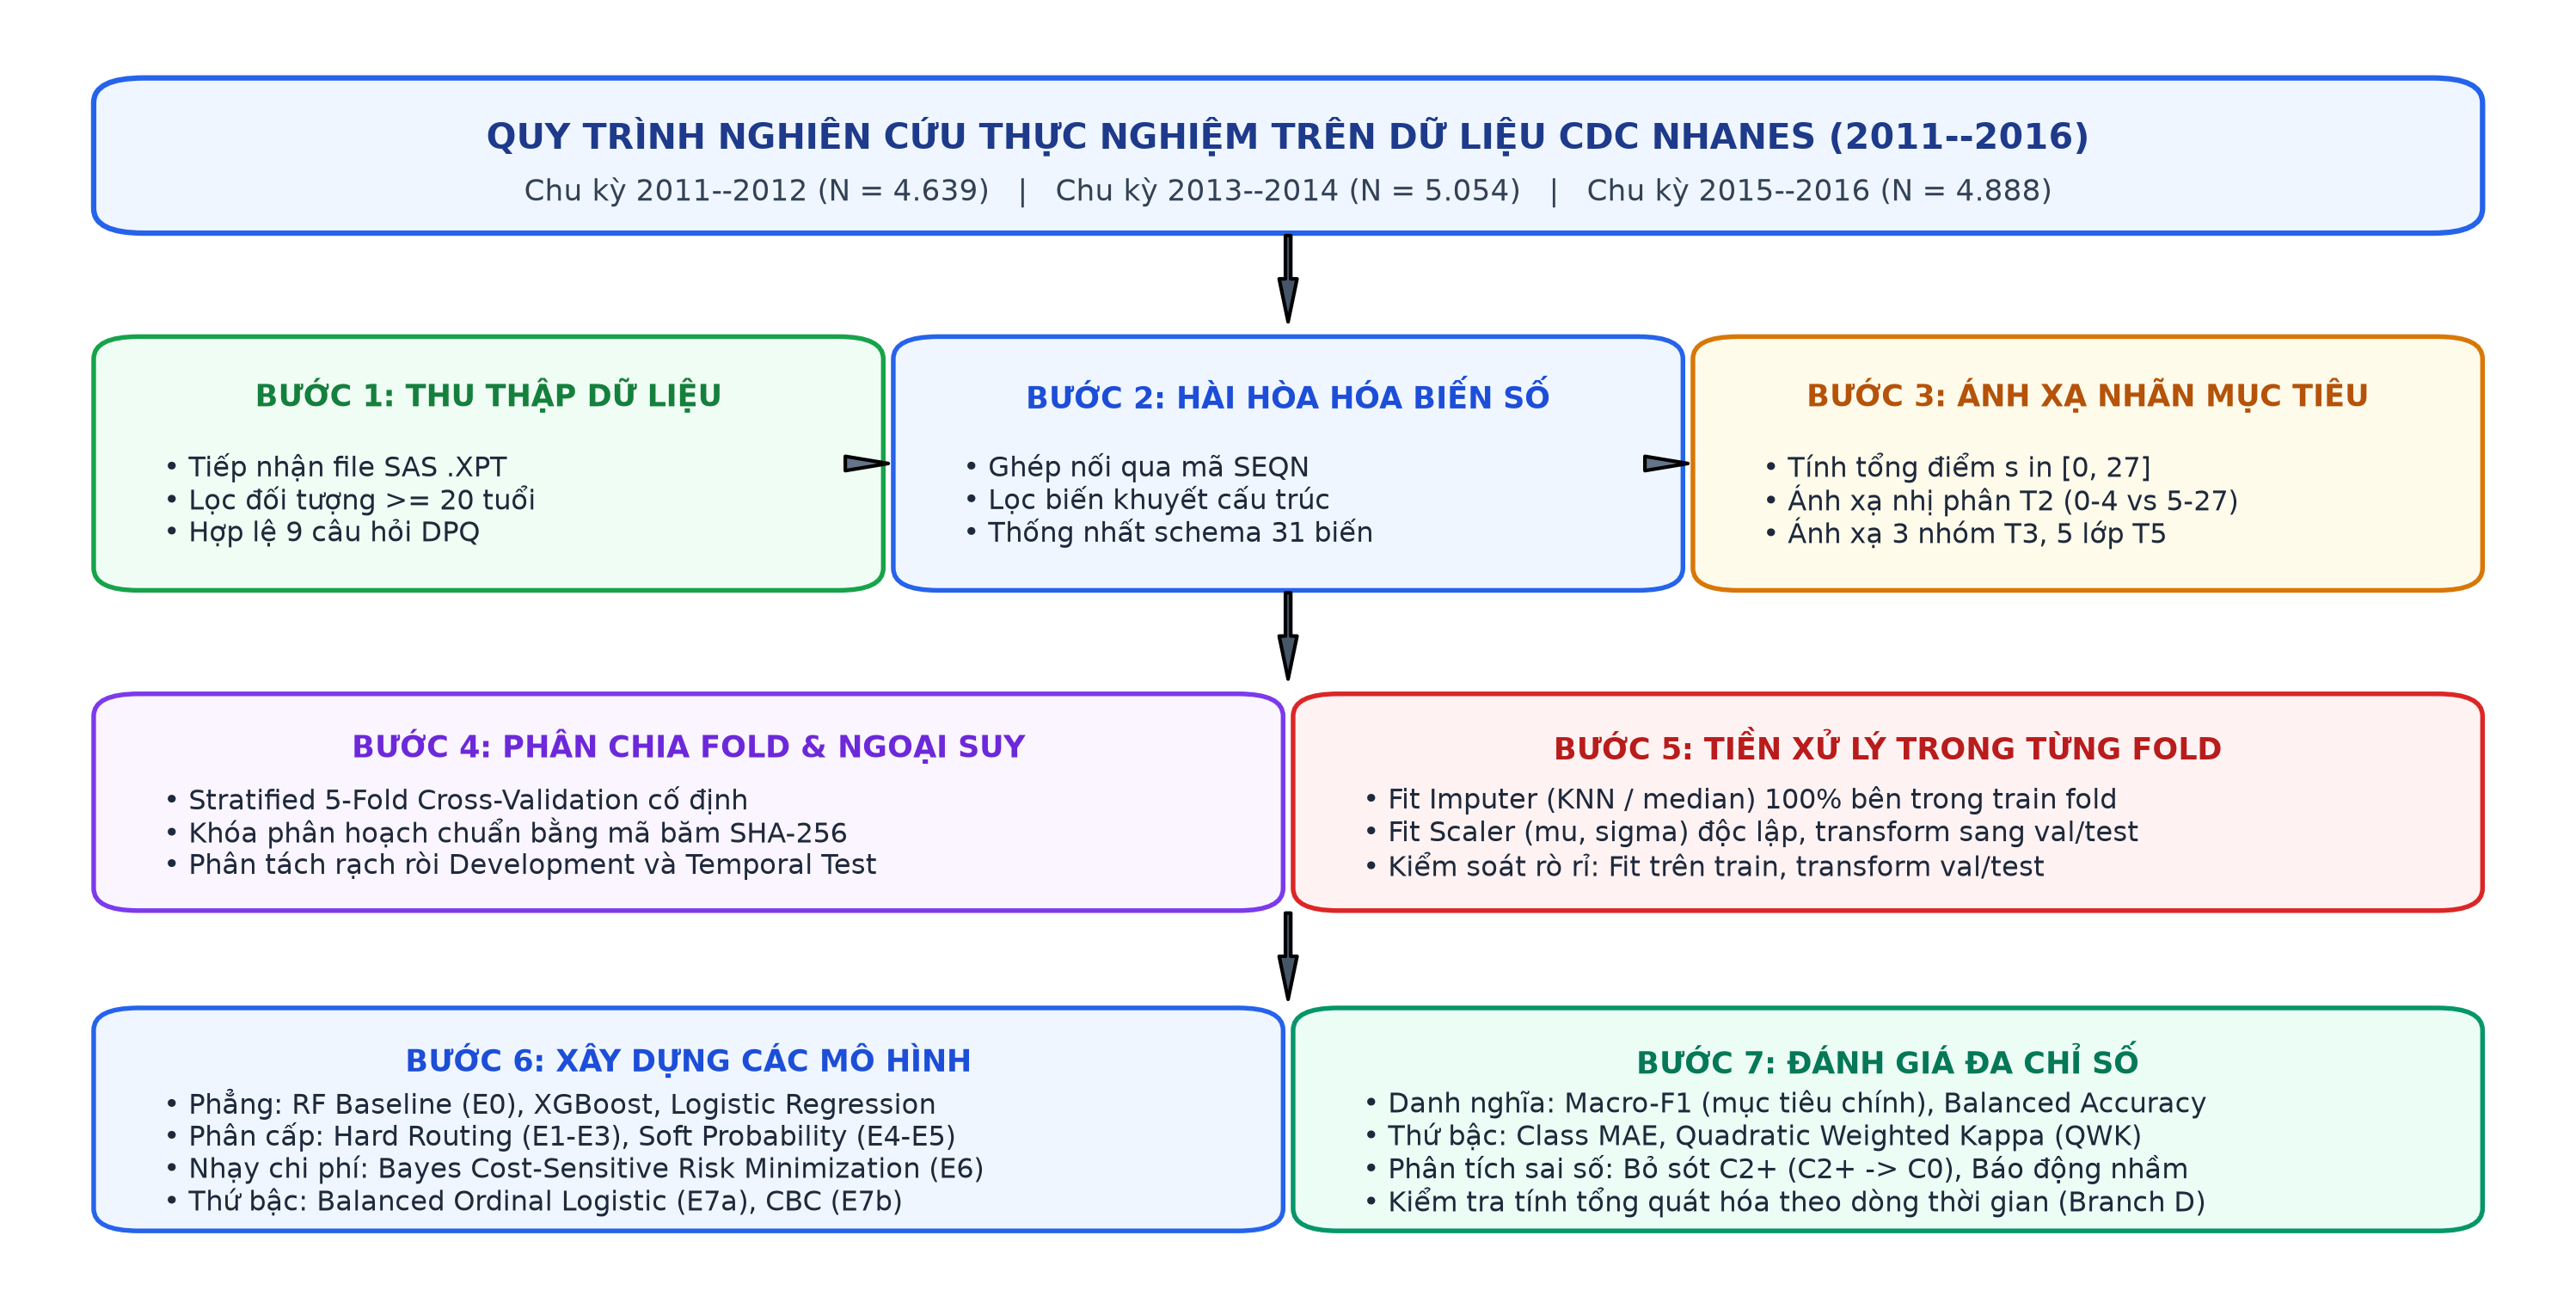
\includegraphics[width=\textwidth]{figures/depsev_overall_architecture.png}
\label{fig:overall-architecture}
\end{figure}
\FloatBarrier

Các bước thực hiện các chức năng cụ thể:
\begin{enumerate}
    \item \textbf{Bước 1 -- Tiếp nhận và lọc đối tượng (Cohort Filtering):} Tiếp nhận các tệp dữ liệu gốc định dạng SAS Transport (.XPT) từ cổng thông tin CDC/NCHS, áp dụng tiêu chuẩn chọn đối tượng người trưởng thành ($\text{RIDAGEYR} \ge 20$) có đầy đủ 9 câu hỏi khảo sát DPQ hợp lệ.
    \item \textbf{Bước 2 -- Hài hòa hóa và trích xuất đặc trưng (Feature Engineering):} Ghép nối các bảng khảo sát và xét nghiệm qua mã định danh SEQN; chuẩn hóa tên biến, xử lý biến điều hướng và loại bỏ các biến có tỷ lệ khuyết thiếu lớn giữa các chu kỳ.
    \item \textbf{Bước 3 -- Thiết lập không gian nhãn mục tiêu (Target Space Mapping):} Ánh xạ tổng điểm PHQ-9 thành 4 không gian mục tiêu rời rạc ($T_2, T_3, T_4, T_5$) phục vụ khảo sát đa độ phân giải.
    \item \textbf{Bước 4 -- Phân hoạch dữ liệu có kiểm soát (Partitioning):} Quản lý các phân hoạch dữ liệu cố định (Stratified 5-Fold CV, Development/Held-out splits) bằng mã băm SHA-256 nhằm bảo đảm tính tái lập thực nghiệm.
    \item \textbf{Bước 5 -- Tiền xử lý dữ liệu in-fold (In-Fold Preprocessing):} Thực hiện quy trình điền khuyết (median/mode), chuẩn hóa (StandardScaler) và mã hóa one-hot độc lập bên trong từng fold huấn luyện để kiểm soát rò rỉ dữ liệu.
    \item \textbf{Bước 6 -- Thử nghiệm các hướng mô hình hóa (Model Zoo):} Triển khai mô hình phân loại phẳng ($E_0$), 4 cấu hình phân cấp cứng ($E_1 \to E_3$), 4 cấu hình phân cấp mềm kết hợp tối ưu chi phí Bayes ($E_4 \to E_6$) và các cấu hình phân loại thứ bậc ($E_7$).
    \item \textbf{Bước 7 -- Đánh giá hiệu năng đa chiều (Evaluation Suite):} Đánh giá hiệu năng qua hệ thống độ đo phân loại danh nghĩa (Macro-F1, Balanced Accuracy), độ đo thứ bậc (Class MAE, Quadratic Weighted Kappa) và số lượng ca nặng bị phân loại nhầm ($C_2^+ \to C_0$).
\end{enumerate}

\section{Bộ dữ liệu NHANES và Quy trình tiền xử lý in-fold}
\label{sec:du-lieu-nghien-cuu}

\subsection{Tập dữ liệu phát triển Legacy (NHANES 2013--2014)}
\label{subsec:legacy-cohort}

Tập dữ liệu Legacy được xây dựng từ chu kỳ NHANES 2013--2014, gồm $N = 5.054$ đối tượng trưởng thành có dữ liệu PHQ-9 hợp lệ:
\begin{itemize}
    \item \textbf{Phân hoạch phát triển (Development Cohort):} Gồm $N = 4.045$ đối tượng, được sử dụng xuyên suốt cho các thực nghiệm Stratified 5-Fold CV, Feature Ablation, Nested Hyperparameter Tuning và chuỗi thực nghiệm chính $E_0 \to E_7$.
    \item \textbf{Phân hoạch kiểm tra bổ sung (Supplementary Held-out Cohort):} Gồm $N = 1.009$ đối tượng được lưu giữ riêng để tham khảo đối chứng. Cần ghi nhận tính chất lịch sử: 813 trong số 1.009 đối tượng này từng nằm trong tập phát triển ở các phiên bản tiền nghiệm, do đó tập này chỉ mang giá trị tham chiếu phụ trợ, toàn bộ kết luận khoa học cốt lõi dựa trên quy trình kiểm định chéo Stratified 5-Fold lồng nhau trên tập phát triển.
\end{itemize}

Phân bố chi tiết các mức độ triệu chứng PHQ-9 trên tập Legacy được tổng hợp trong Bảng \ref{tab:legacy-class-dist}. Tỷ lệ lớp thiểu số rất nặng $C_4$ chỉ chiếm 1.09\%, thể hiện tính chất mất cân bằng của bài toán.

\begin{table}{Phân bố các lớp triệu chứng PHQ-9 trên tập dữ liệu Legacy ($N = 5.054$)}
\centering
\footnotesize
\setlength{\tabcolsep}{3pt}
\label{tab:legacy-class-dist}
\begin{tabularx}{\textwidth}{l c >{\centering\arraybackslash}X >{\centering\arraybackslash}X >{\centering\arraybackslash}X >{\centering\arraybackslash}X >{\centering\arraybackslash}X}
\toprule
\textbf{Phân hoạch} & \textbf{Tổng $N$} & \textbf{$C_0$ (0--4)} & \textbf{$C_1$ (5--9)} & \textbf{$C_2$ (10--14)} & \textbf{$C_3$ (15--19)} & \textbf{$C_4$ (20--27)} \\
\midrule
Development & 4.045 & 3.016 (74.56\%) & 638 (15.77\%) & 243 (6.01\%) & 104 (2.57\%) & 44 (1.09\%) \\
Held-out & 1.009 & 748 (74.13\%) & 162 (16.06\%) & 60 (5.95\%) & 28 (2.78\%) & 11 (1.09\%) \\
\midrule
\textbf{Toàn bộ} & \textbf{5.054} & \textbf{3.764 (74.48\%)} & \textbf{800 (15.83\%)} & \textbf{303 (6.00\%)} & \textbf{132 (2.61\%)} & \textbf{55 (1.09\%)} \\
\bottomrule
\end{tabularx}
\end{table}

\subsection{Tập dữ liệu đa chu kỳ chính thức (Official Multi-Cycle Cohort)}
\label{subsec:multicycle-cohort}

Để kiểm tra tính ổn định trên quy mô lớn và đánh giá khả năng tổng quát hóa theo dòng thời gian, nghiên cứu tiến hành trích xuất và hài hòa hóa dữ liệu từ ba chu kỳ NHANES liên tiếp: 2011--2012, 2013--2014 và 2015--2016, nâng tổng quy mô lên $N = 14.581$ đối tượng (Bảng \ref{tab:multicycle-class-dist}).

\begin{table}{Quy mô và phân bố các lớp triệu chứng trên các chu kỳ NHANES chính thức}
\centering
\footnotesize
\setlength{\tabcolsep}{3pt}
\label{tab:multicycle-class-dist}
\begin{tabularx}{\textwidth}{l c >{\centering\arraybackslash}X >{\centering\arraybackslash}X >{\centering\arraybackslash}X >{\centering\arraybackslash}X >{\centering\arraybackslash}X}
\toprule
\textbf{Chu kỳ / Phân nhánh} & \textbf{Tổng $N$} & \textbf{$C_0$ (\%)} & \textbf{$C_1$ (\%)} & \textbf{$C_2$ (\%)} & \textbf{$C_3$ (\%)} & \textbf{$C_4$ (\%)} \\
\midrule
NHANES 2011--2012 & 4.639 & 76.12\% & 14.79\% & 5.22\% & 2.61\% & 1.27\% \\
NHANES 2013--2014 (Branch A) & 5.054 & 74.48\% & 15.83\% & 6.00\% & 2.61\% & 1.09\% \\
NHANES 2015--2016 (Branch D Test) & 4.888 & 74.65\% & 17.21\% & 5.03\% & 2.03\% & 1.08\% \\
\midrule
\textbf{Pooled 2011--2016 (Branch B)} & \textbf{14.581} & \textbf{75.06\%} & \textbf{15.96\%} & \textbf{5.42\%} & \textbf{2.41\%} & \textbf{1.15\%} \\
\bottomrule
\end{tabularx}
\end{table}

\subsection{Quy trình tiền xử lý và kiểm soát rò rỉ dữ liệu in-fold}
\label{subsec:data-pipeline}

Quy trình tiền xử lý và hài hòa hóa dữ liệu được thực hiện như trình bày trong Hình \ref{fig:data-pipeline}.

\begin{figure}[htbp]{Quy trình tiền xử lý dữ liệu in-fold và kiểm soát rò rỉ dữ liệu}
\centering
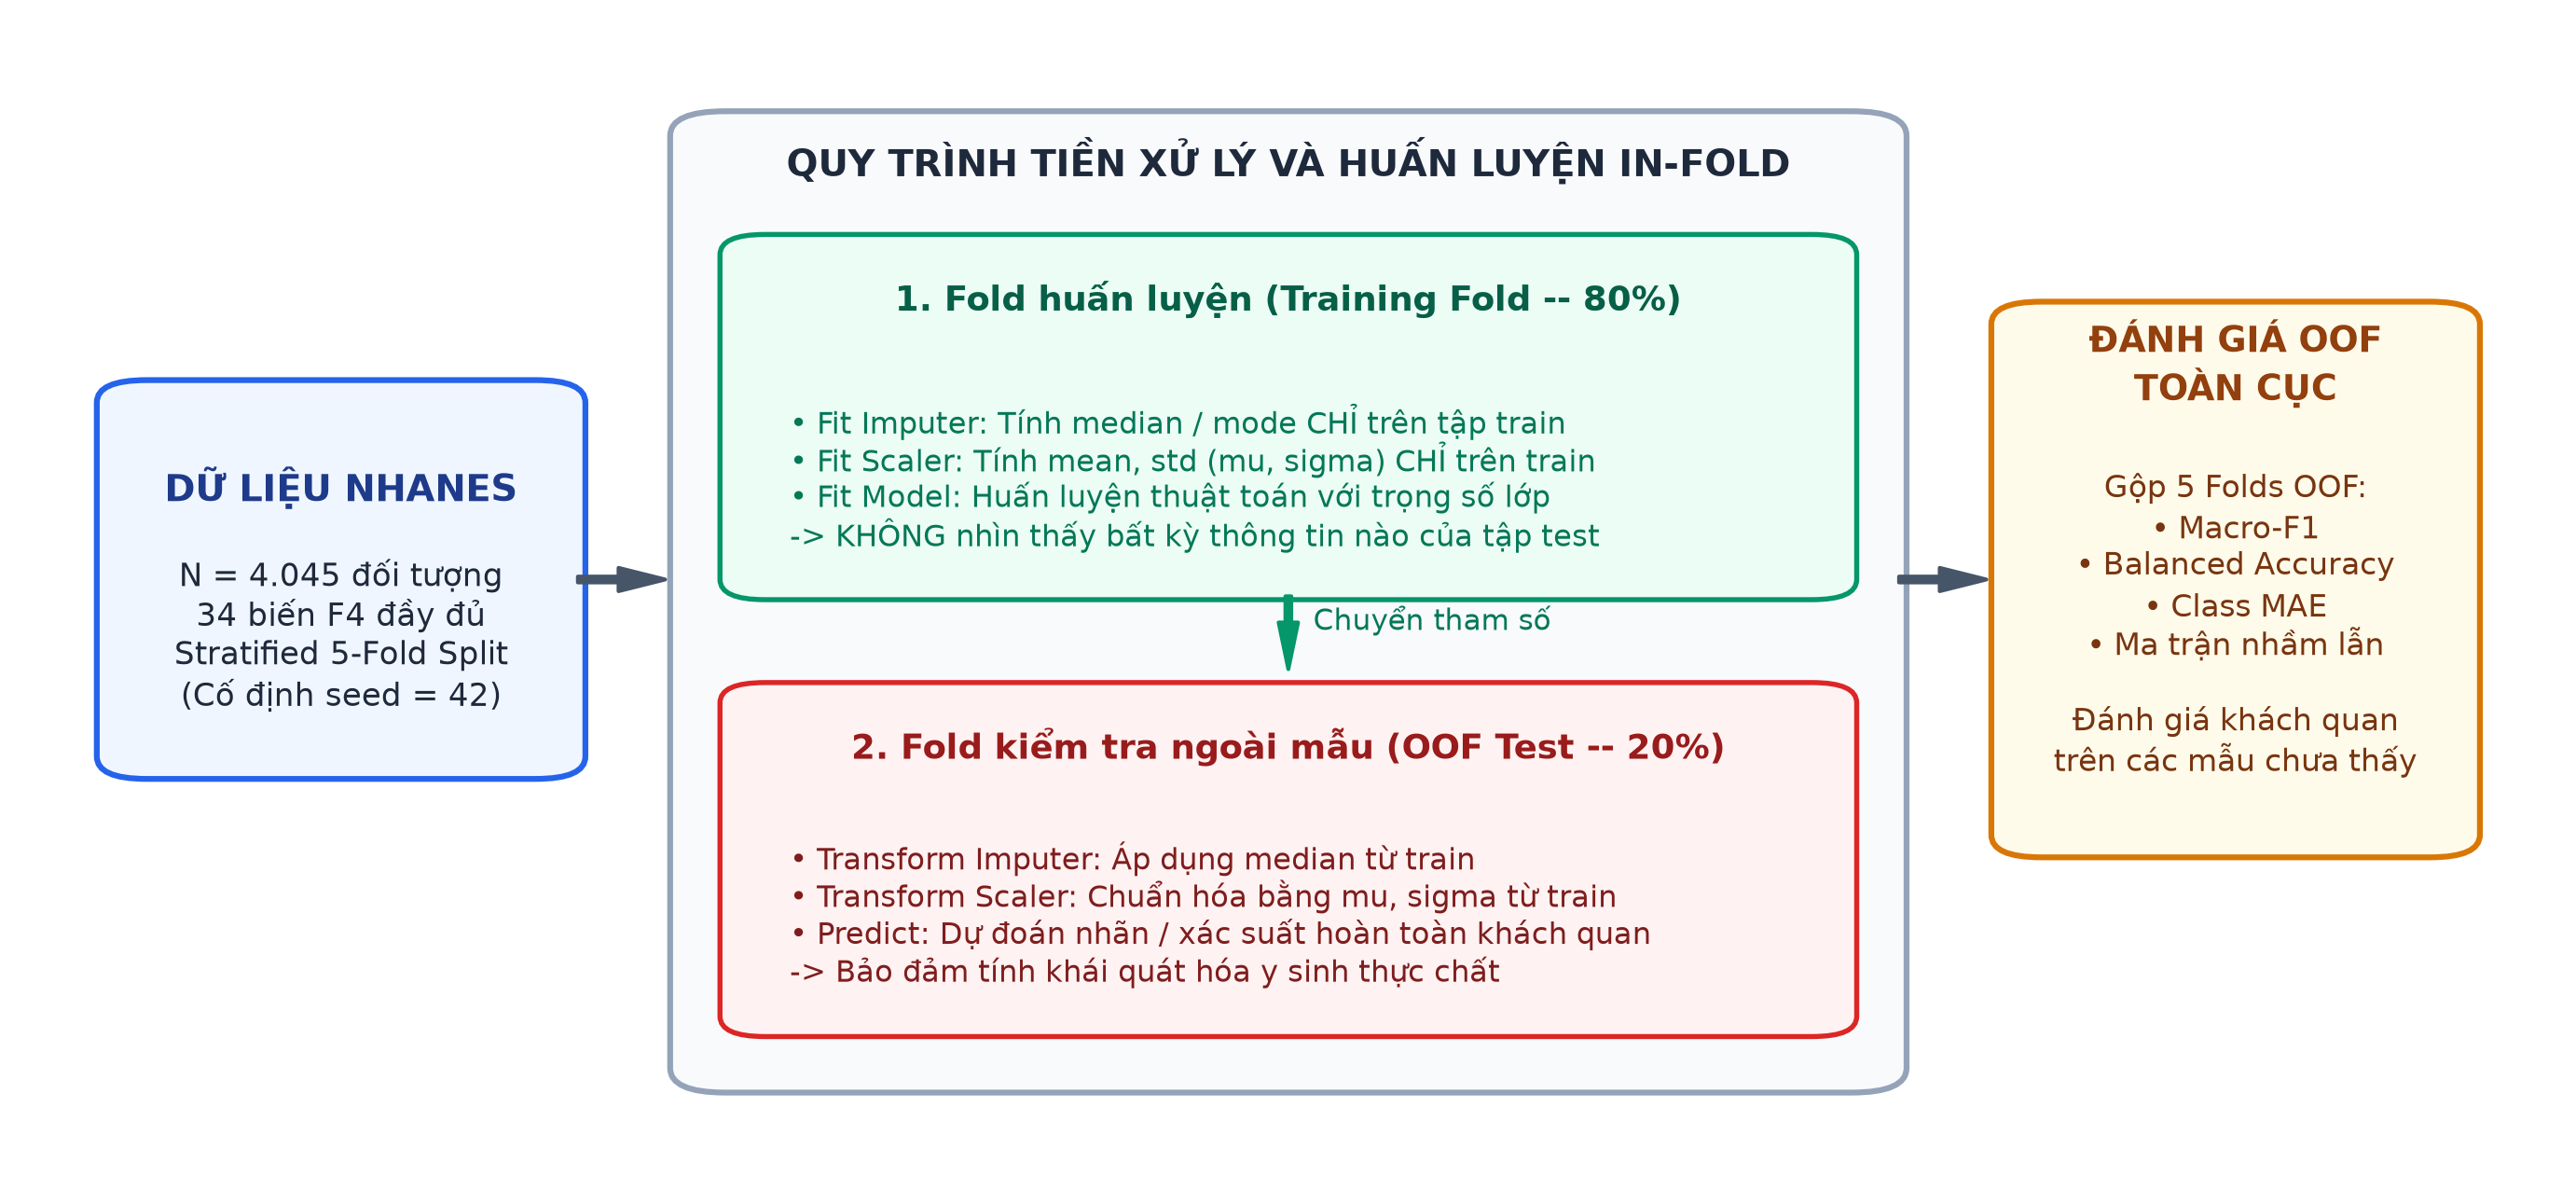
\includegraphics[width=\textwidth]{figures/fig3_infold_cv_pipeline.png}
\label{fig:data-pipeline}
\end{figure}
\FloatBarrier

Quy trình bảo đảm các yêu cầu kỹ thuật:
\begin{enumerate}
    \item \textbf{Loại trừ biến khuyết cấu trúc:} Biến xét nghiệm Triglyceride chỉ lấy mẫu trên nhóm nhịn ăn sáng ở một số chu kỳ (khuyết thiếu > 50\%), nên được loại bỏ để bảo đảm tính tương thích của 31 đặc trưng cốt lõi ($F_{4\_\text{common31}}$).
    \item \textbf{Cô lập tham số in-fold:} Các giá trị thống kê phục vụ điền khuyết (trung vị cho biến liên tục, mode cho biến phân loại) và tham số chuẩn hóa phương sai ($\mu, \sigma$ của \texttt{StandardScaler}) được tính độc lập trên tập huấn luyện của fold hiện tại, sau đó áp dụng biến đổi cho fold kiểm tra.
    \item \textbf{Bảo toàn nhãn mục tiêu:} Không đưa bất kỳ câu hỏi nào trong 9 mục khảo sát DPQ vào ma trận đặc trưng đầu vào $\mathbf{X}$.
\end{enumerate}

\section{Xây dựng không gian đặc trưng lũy tiến ($F_1 \to F_4$)}
\label{sec:he-thong-dac-trung}

Để khảo sát thực nghiệm mức độ đóng góp của từng nhóm biến số (RQ1), DepSev-ML tổ chức 34 biến đầu vào thành 4 không gian đặc trưng lũy tiến ($F_1 \to F_4$) như mô tả trong Hình \ref{fig:feature-groups}.

\begin{figure}[htbp]{Cấu trúc 4 không gian đặc trưng lũy tiến $F_1 \to F_4$ trong DepSev-ML}
\centering
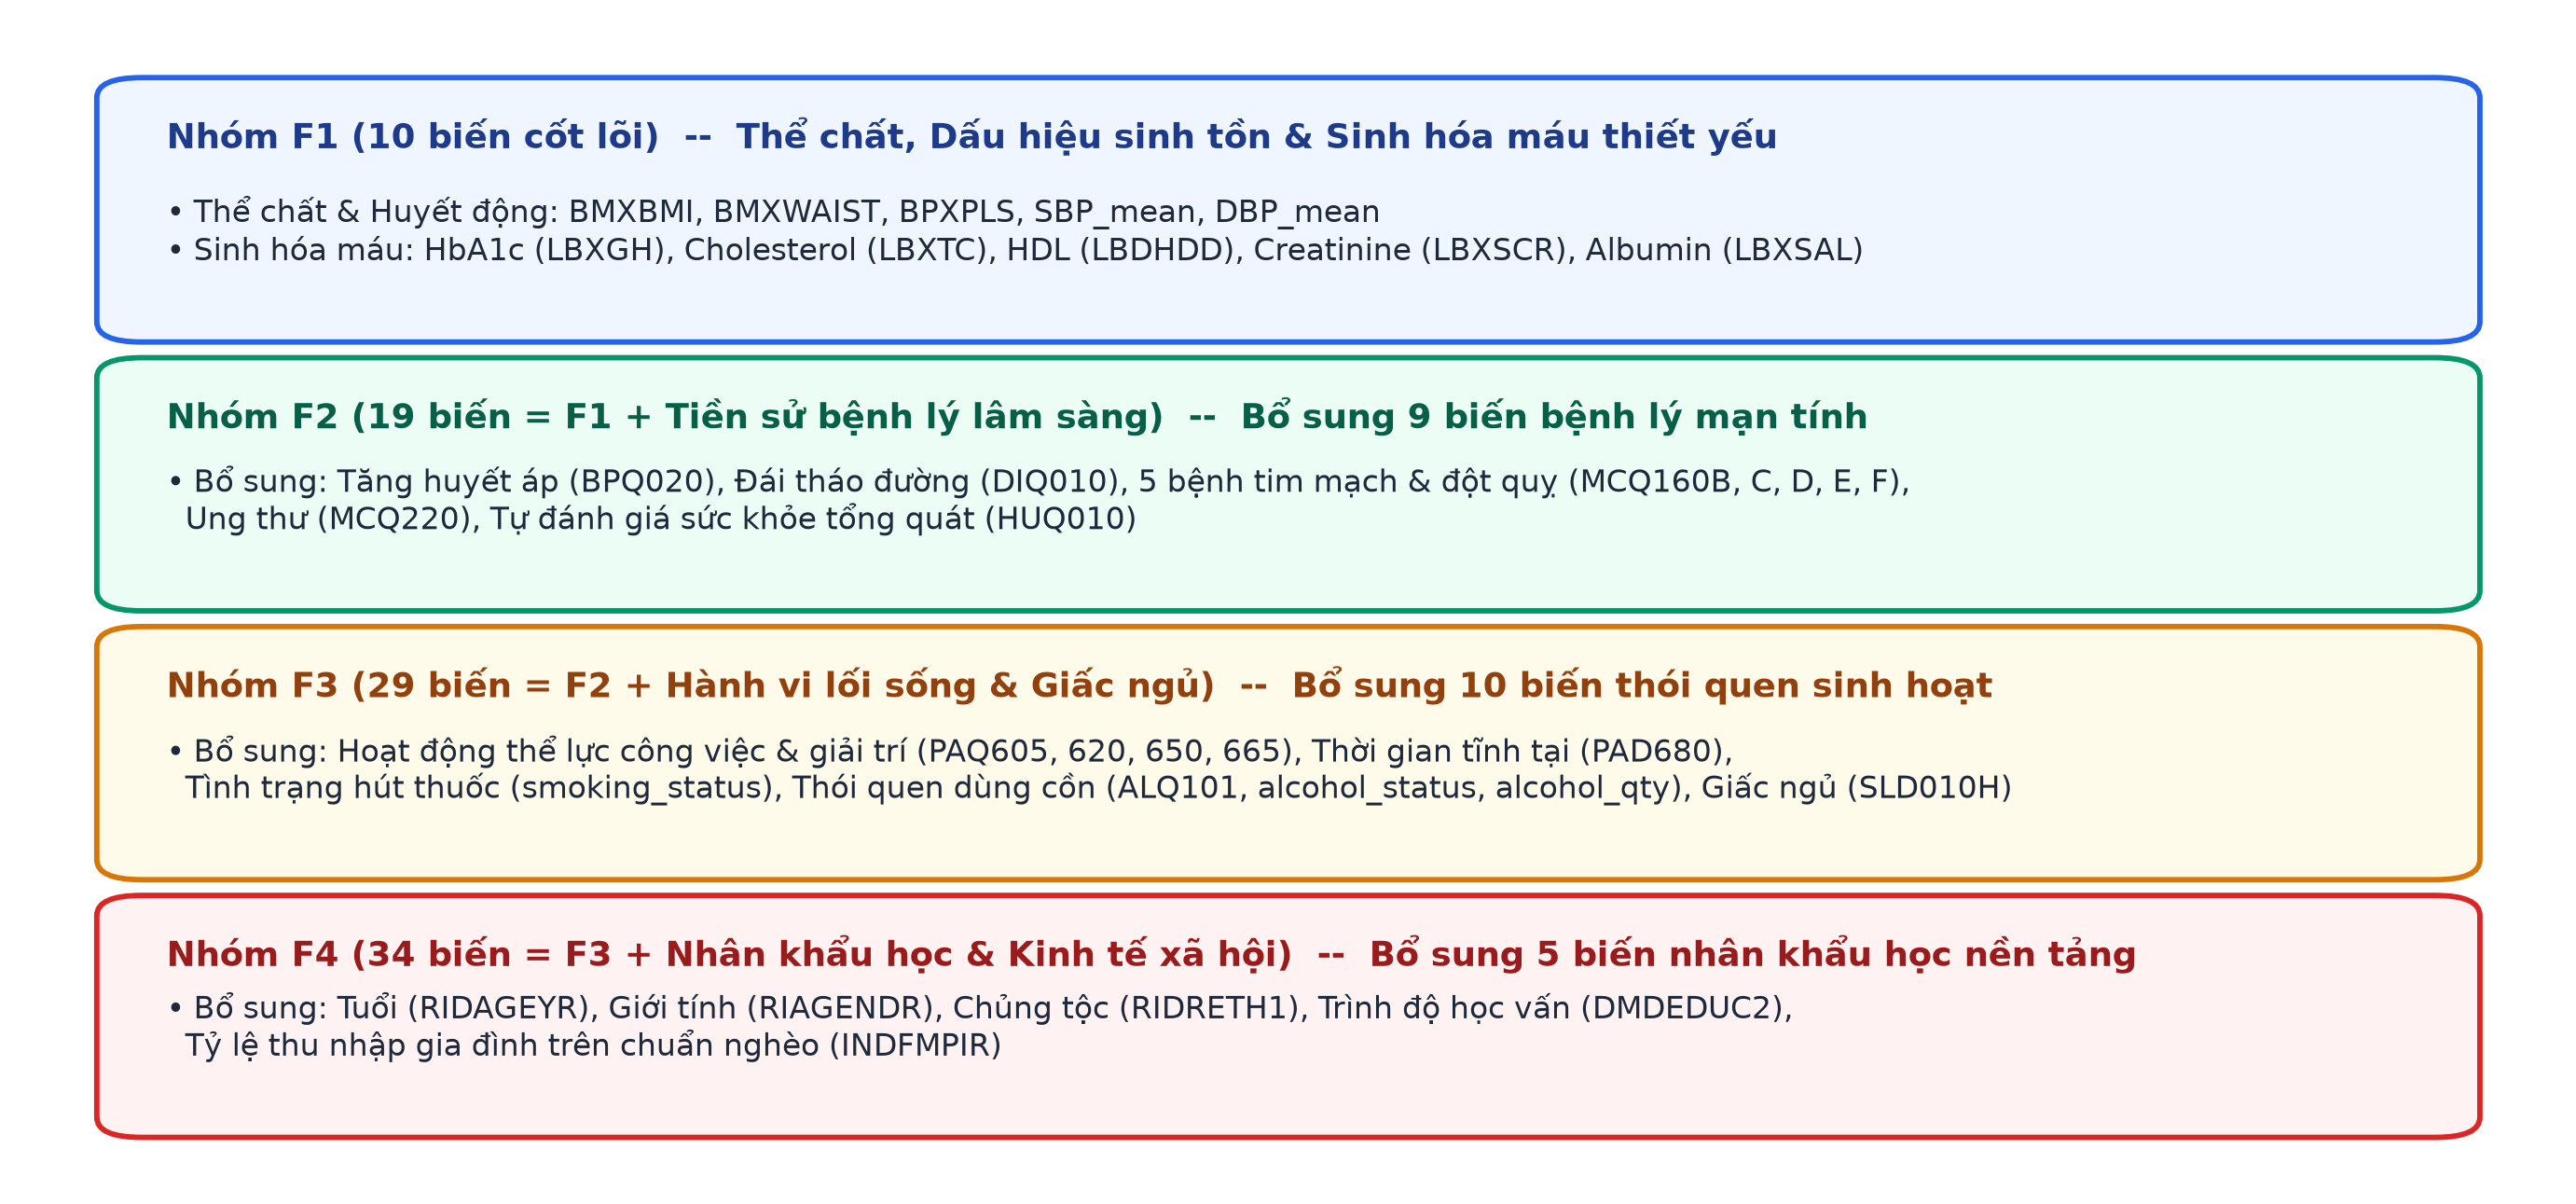
\includegraphics[width=\textwidth]{figures/fig3_3_feature_groups.png}
\label{fig:feature-groups}
\end{figure}
\FloatBarrier

Các không gian đặc trưng gồm:
\begin{itemize}
    \item \textbf{Không gian $F_1$ (10 biến cốt lõi):} Gồm 5 chỉ số thể chất và huyết áp (BMI, chu vi vòng eo, nhịp tim nghỉ, huyết áp tâm thu trung bình, huyết áp tâm trương trung bình) kết hợp 5 chỉ số sinh hóa máu (HbA1c, Cholesterol toàn phần, HDL, Creatinine và Albumin).
    \item \textbf{Không gian $F_2$ (19 biến = $F_1$ + Tiền sử bệnh lý):} Bổ sung 9 biến tiền sử bệnh mạn tính: tăng huyết áp, đái tháo đường, 5 bệnh lý tim mạch và đột quỵ, tiền sử ung thư và tự đánh giá sức khỏe.
    \item \textbf{Không gian $F_3$ (29 biến = $F_2$ + Lối sống \& Giấc ngủ):} Bổ sung 10 chỉ số hành vi: hoạt động thể lực tại nơi làm việc và giải trí, thời gian tĩnh tại, tình trạng hút thuốc, thói quen uống rượu bia và thời lượng giấc ngủ.
    \item \textbf{Không gian $F_4$ (34 biến = $F_3$ + Nhân khẩu học \& Kinh tế xã hội):} Bổ sung 5 biến nhân khẩu học: tuổi, giới tính, chủng tộc, học vấn và tỷ lệ thu nhập gia đình trên chuẩn nghèo (INDFMPIR).
\end{itemize}

Bảng \ref{tab:feature-summary} tóm tắt cấu trúc phân nhóm đặc trưng; danh mục chi tiết 34 biến kèm mã định danh CDC được trình bày tại Phụ lục \ref{app:feature-inventory}.

\begin{table}{Tóm tắt cấu trúc 4 không gian đặc trưng lũy tiến trong DepSev-ML}
\centering
\footnotesize
\setlength{\tabcolsep}{4pt}
\label{tab:feature-summary}
\begin{tabularx}{\textwidth}{l c p{5.5cm} X}
\toprule
\textbf{Không gian} & \textbf{Số biến} & \textbf{Các nhóm biến thành phần} & \textbf{Ý nghĩa lâm sàng và dịch tễ học} \\
\midrule
$F_1$ & 10 & Thể chất, Sinh tồn \& Xét nghiệm máu thiết yếu & Phản ánh chuyển hóa cơ bản, huyết động và viêm mạn tính \\
$F_2$ & 19 & $F_1$ + 9 tiền sử bệnh lý mạn tính & Tích hợp chẩn đoán tiền sử của bác sĩ và tự đánh giá sức khỏe \\
$F_3$ & 29 & $F_2$ + 10 hành vi lối sống \& giấc ngủ & Bổ sung nhịp sinh học, mức độ vận động và hành vi kích thích \\
$F_4$ & 34 & $F_3$ + 5 nhân khẩu học \& kinh tế xã hội & Bổ sung yếu tố nguy cơ xã hội, độ tuổi và áp lực kinh tế \\
\midrule
$F_{4\_\text{common31}}$ & 31 & 31 biến đồng nhất trên cả 3 chu kỳ NHANES & Chuẩn hóa schema phục vụ kiểm định đa chu kỳ Pooled \\
\bottomrule
\end{tabularx}
\end{table}

\section{Xây dựng nhãn PHQ-9 và các không gian mục tiêu ($T_2 \to T_5$)}
\label{sec:nhan-muc-tieu}

Từ tổng điểm PHQ-9 liên tục $s \in [0, 27]$, nghiên cứu thiết lập 4 không gian phân loại mục tiêu:
\begin{itemize}
    \item $T_2$ ($K=2$): Nhị phân giữa $C_0$ ($s \in [0, 4]$) và nhóm có triệu chứng ($s \in [5, 27]$).
    \item $T_3$ ($K=3$): Ba nhóm gộp quy ước gồm $C_0$ ($0$--$4$, 74.6\%), $C_1$ ($5$--$9$, 15.8\%) và $C_2^+$ ($10$--$27$, 9.7\%). Nhóm $C_2^+$ được quy ước là "nhóm Nặng theo quy ước nghiên cứu" (Severe convention) bao gồm toàn bộ các ca từ Moderate đến Severe chuẩn.
    \item $T_4$ ($K=4$): Bốn mức gồm $C_0$ ($0$--$4$), $C_1$ ($5$--$9$), $C_2$ ($10$--$14$), và $C_3^+$ ($15$--$27$).
    \item $T_5$ ($K=5$): Năm mức độ lâm sàng chuẩn PHQ-9 gồm $C_0$ (Minimal), $C_1$ (Mild), $C_2$ (Moderate), $C_3$ (Moderately severe), và $C_4$ (Severe).
\end{itemize}

\section{Quy trình áp dụng Random Forest trên dữ liệu thực tế NHANES}
\label{sec:xay-dung-random-forest}

Random Forest đóng vai trò là mô hình học máy cơ sở chính trong toàn bộ khung nghiên cứu DepSev-ML. Quy trình phát triển, huấn luyện và kiểm định mô hình Random Forest trên dữ liệu NHANES gồm các bước:

\begin{enumerate}
    \item \textbf{Bước 1 -- Xác lập tập dữ liệu và không gian đặc trưng:} 
    Mô hình được áp dụng trên tập dữ liệu phát triển Legacy gồm $N = 4.045$ đối tượng với không gian 34 đặc trưng đầy đủ ($F_4$). Phân phối nhãn 5 lớp mất cân bằng rõ rệt: $C_0$ chiếm $3.016$ ca (74.56\%), $C_1$ chiếm $638$ ca (15.77\%), $C_2$ chiếm $243$ ca (6.01\%), $C_3$ chiếm $104$ ca (2.57\%) và $C_4$ chỉ có $44$ ca (1.09\%).
    
    \item \textbf{Bước 2 -- Thiết lập phân hoạch Stratified 5-Fold Cross-Validation:} 
    Dữ liệu được phân chia thành 5 folds bằng cơ chế Stratified cố định hạt giống ngẫu nhiên \texttt{random\_state = 42}, bảo đảm tỷ lệ giữa các lớp nhãn tương đồng giữa tập huấn luyện (4 folds, $\approx 3.236$ mẫu) và tập kiểm định (1 fold, $\approx 809$ mẫu). Cấu trúc kiểm định lồng nhau (Nested CV: Outer 5 folds, Inner 3 folds) được thiết lập để tìm kiếm siêu tham số mà không tiếp xúc với tập kiểm tra của fold ngoài.
    
    \item \textbf{Bước 3 -- Thực hiện tiền xử lý in-fold kiểm soát rò rỉ dữ liệu:} 
    Để kiểm soát nguy cơ rò rỉ dữ liệu (Hình \ref{fig:data-pipeline}), quy trình điền khuyết giá trị thiếu (median cho biến liên tục, mode cho biến phân loại) và chuẩn hóa phân phối (\texttt{StandardScaler}) được tính toán độc lập bên trong từng fold huấn luyện, sau đó áp dụng lên fold kiểm định.
    
    \item \textbf{Bước 4 -- Cấu hình siêu tham số cố định (Frozen RF Spec):} 
    Bộ tham số thu được từ Nested CV được cố định: \texttt{n\_estimators = 150}, \texttt{max\_depth = 8}, \texttt{max\_features = 0.5}, \texttt{min\_samples\_split = 10}, \texttt{min\_samples\_leaf = 8}, \texttt{criterion = 'gini'}, \texttt{random\_state = 42}. Tham số \texttt{class\_weight = 'balanced\_subsample'} được kích hoạt để tự động điều chỉnh trọng số nghịch đảo tần số lớp trên từng mẫu bootstrap riêng biệt của mỗi cây.
    
    \item \textbf{Bước 5 -- Huấn luyện và suy luận Soft Voting:} 
    Tập hợp $150$ cây quyết định được huấn luyện độc lập trên các tập con bootstrap. Khi suy luận trên fold kiểm định, mẫu dữ liệu được đưa qua toàn bộ $150$ cây và xuất ra phân phối xác suất trung bình liên tục (Soft Voting): $\bar{P}(Y = k \mid \mathbf{x}) = \frac{1}{150}\sum_{b=1}^{150} P_b(Y = k \mid \mathbf{x})$.
    
    \item \textbf{Bước 6 -- Đánh giá hiệu năng và phân tích hạn chế:} 
    Mô hình được đánh giá qua các chỉ số: Macro-F1, Balanced Accuracy, Weighted-F1, Brier Score và Class MAE. Kết quả thực nghiệm chi tiết của Random Forest trên bài toán 5 lớp $T_5$, phân tích ma trận nhầm lẫn và sự suy thoái của lớp trung gian $C_1$ sẽ được trình bày tại Chương \ref{ch:thuc-nghiem}. Những hạn chế cốt lõi quan sát được trên $T_5$ là động lực để nghiên cứu mở rộng sang bài toán phân cấp hai giai đoạn $T_3$.
\end{enumerate}

\section{Thiết kế các kiến trúc phân loại phân cấp hai giai đoạn ($T_3$) và các mô hình mở rộng ($E_0 \to E_7$)}
\label{sec:thiet-ke-kien-truc-mo-hinh}

Từ hiện tượng chồng lấn phân phối và sự suy giảm khả năng nhận diện của lớp $C_1$ khi phân loại 5 lớp phẳng trên $T_5$, nghiên cứu chuyển hướng sang bài toán 3 nhóm ($T_3$: $C_0, C_1, C_2^+$). Trên không gian $T_3$, nghiên cứu khảo sát và so sánh 8 cấu hình mô hình thực nghiệm ($E_0 \to E_7$).

\subsection{Mô hình phân loại phẳng cơ sở ($E_0$)}
\label{subsec:e0-flat}

Mô hình $E_0$ sử dụng thuật toán Random Forest đa lớp truyền thống làm đường cơ sở đối chuẩn trên không gian 3 nhóm ($C_0, C_1, C_2^+$). Dự đoán đầu ra là lớp có xác suất hậu nghiệm cực đại: $\hat{y} = \arg\max_k P(Y=k \mid \mathbf{x})$.

\subsection{Kiến trúc phân loại phân cấp hai giai đoạn định tuyến cứng ($E_1 \to E_3$)}
\label{subsec:hard-hierarchical}

Kiến trúc phân cấp hai giai đoạn phân rã bài toán 3 lớp thành hai bộ phân loại nhị phân nối tiếp (Hình \ref{fig:hard-hierarchical}):
\begin{itemize}
    \item \textbf{Giai đoạn 1 (Bộ phân loại sàng lọc $M_1$):} Phân loại nhị phân phát hiện đối tượng có triệu chứng, phân biệt giữa nhóm triệu chứng tối thiểu ($C_0$, điểm PHQ-9 $0$--$4$) và nhóm có triệu chứng ($C_{12} = C_1 \cup C_2^+$, điểm PHQ-9 $5$--$27$).
    \item \textbf{Giai đoạn 2 (Bộ phân loại phân tầng $M_2$):} Trong số các đối tượng có triệu chứng, tiếp tục phân biệt giữa mức độ nhẹ ($C_1$, điểm PHQ-9 $5$--$9$) và mức độ nặng theo quy ước nghiên cứu ($C_2^+$, điểm PHQ-9 $10$--$27$).
\end{itemize}

\begin{figure}[htbp]{Kiến trúc phân loại phân cấp định tuyến cứng hai giai đoạn và điểm nghẽn lan truyền sai số}
\centering
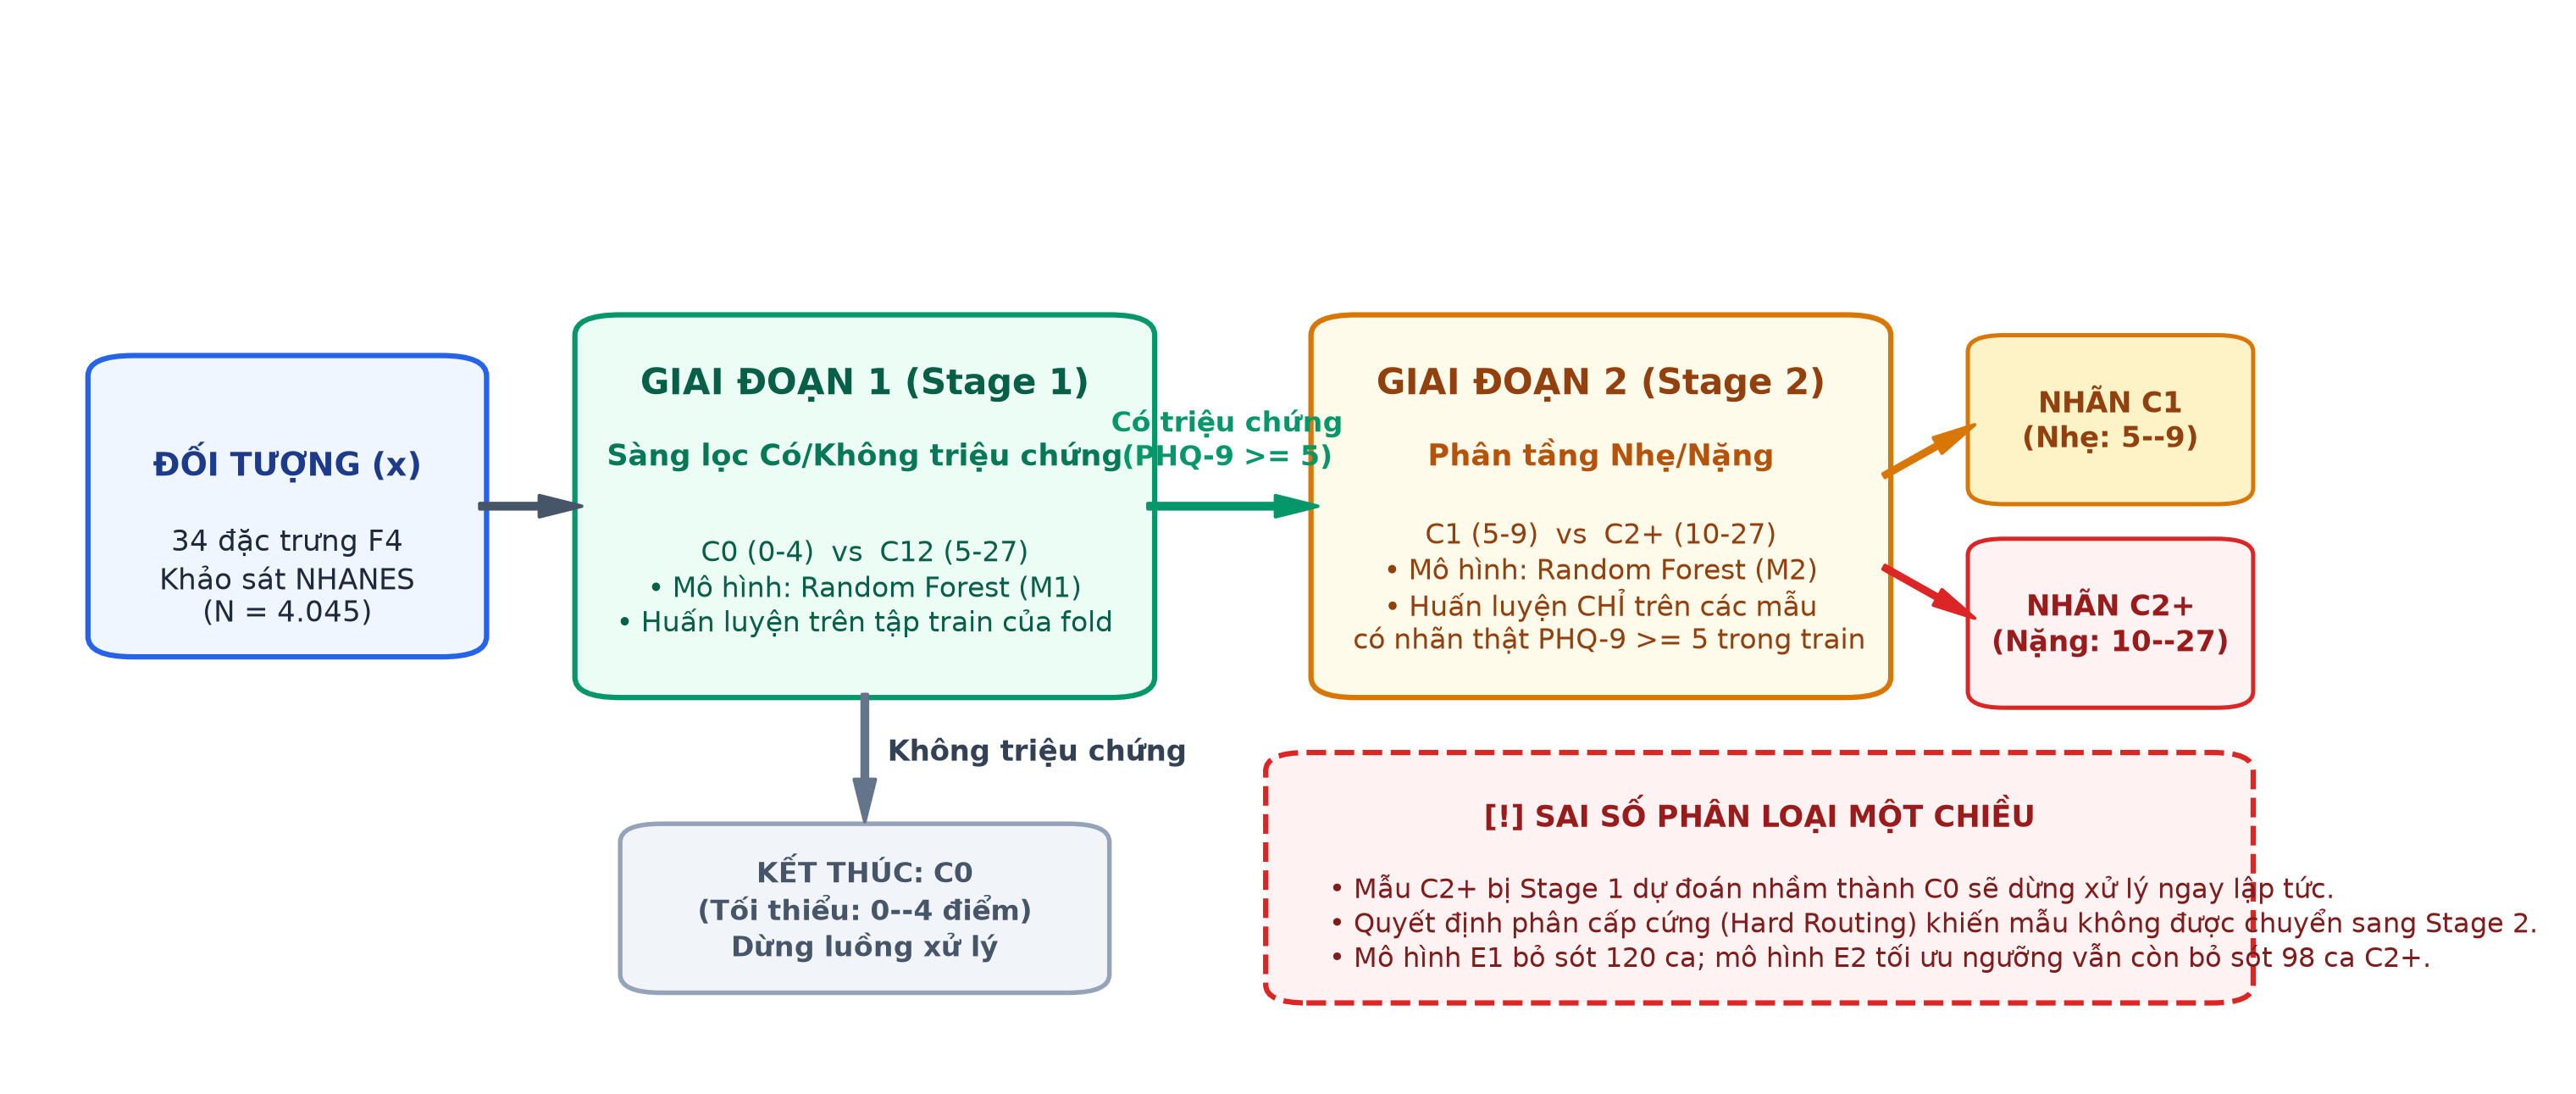
\includegraphics[width=\textwidth]{figures/fig3_4_hard_hierarchical.png}
\label{fig:hard-hierarchical}
\end{figure}
\FloatBarrier

\textbf{Quy trình huấn luyện trong từng fold của Nested Cross-Validation:}
\begin{itemize}
    \item \textbf{Mô hình Stage 1 ($M_1$):} Trong mỗi fold kiểm định chéo, mô hình Stage 1 được huấn luyện trên \textbf{toàn bộ phần dữ liệu huấn luyện của fold đó} ($\approx 3.236$ mẫu trong số tổng $N = 4.045$ mẫu của tập phát triển).
    \item \textbf{Mô hình Stage 2 ($M_2$):} Mô hình Stage 2 được huấn luyện \textbf{chỉ trên các mẫu trong fold huấn luyện có nhãn thật $\text{PHQ-9} \ge 5$} ($\approx 823$ mẫu trong số tổng $1.029$ mẫu có triệu chứng của tập phát triển). Việc giới hạn tập huấn luyện này giúp mô hình $M_2$ học ranh giới phân biệt giữa ca nhẹ và ca nặng mà không bị chi phối bởi lớp đa số $C_0$.
\end{itemize}

\noindent\textbf{Lưu ý về bản chất độc lập của các mô hình và bài toán:} Cần lưu ý rằng mô hình Random Forest trong bài toán 5 lớp phẳng $T_5$, mô hình RF Stage 1 trong $T_3$ và mô hình RF Stage 2 trong $T_3$ là \textbf{các mô hình độc lập, giải quyết các mục tiêu khác nhau và huấn luyện trên các tập dữ liệu khác nhau}. Đồng thời, bài toán $T_3$ là một bài toán phân loại độc lập với không gian nhãn được tái cấu trúc, không phải là kết quả cải thiện trực tiếp trên cùng không gian 5 lớp.

Bốn cấu hình thực nghiệm phân cấp cứng được khảo sát:
\begin{itemize}
    \item $E_1$: Cấu hình Random Forest nối tiếp (RF--RF) với siêu tham số mặc định.
    \item $E_2$: Cấu hình RF--RF tối ưu hóa siêu tham số và ngưỡng cắt độc lập trên từng giai đoạn.
    \item $E_{3a}$: Cấu hình kết hợp RF--LR (Stage 1 dùng RF, Stage 2 dùng Logistic Regression) để kiểm tra mô hình tuyến tính trong không gian mẫu có triệu chứng.
    \item $E_{3b}$: Cấu hình kết hợp RF--XGBoost (Stage 1 dùng RF, Stage 2 dùng XGBoost) nhằm khảo sát khả năng tăng cường độ dốc trên các ca có triệu chứng.
\end{itemize}

\textbf{Điểm nghẽn lan truyền sai số (Error Propagation):} Do quyết định ở Giai đoạn 1 là quyết định cứng, bất kỳ đối tượng nào thuộc nhóm nặng $C_2^+$ bị $M_1$ xếp nhầm thành $C_0$ sẽ bị gán nhãn $C_0$ ngay lập tức và không được $M_2$ xem xét. Đây là hạn chế lớn của cơ chế định tuyến cứng.

\subsection{Kiến trúc phân loại phân cấp định tuyến mềm và tối ưu chi phí Bayes ($E_4 \to E_6$)}
\label{subsec:soft-cost-hierarchical}

Để khắc phục hiện tượng sai số một chiều của định tuyến cứng, kiến trúc phân cấp mềm (Hình \ref{fig:soft-cost-architecture}) chuyển toàn bộ quá trình ra quyết định sang miền xác suất liên tục.

\begin{figure}[htbp]{Kiến trúc phân loại phân cấp mềm kết hợp lý thuyết quyết định nhạy chi phí Bayes}
\centering
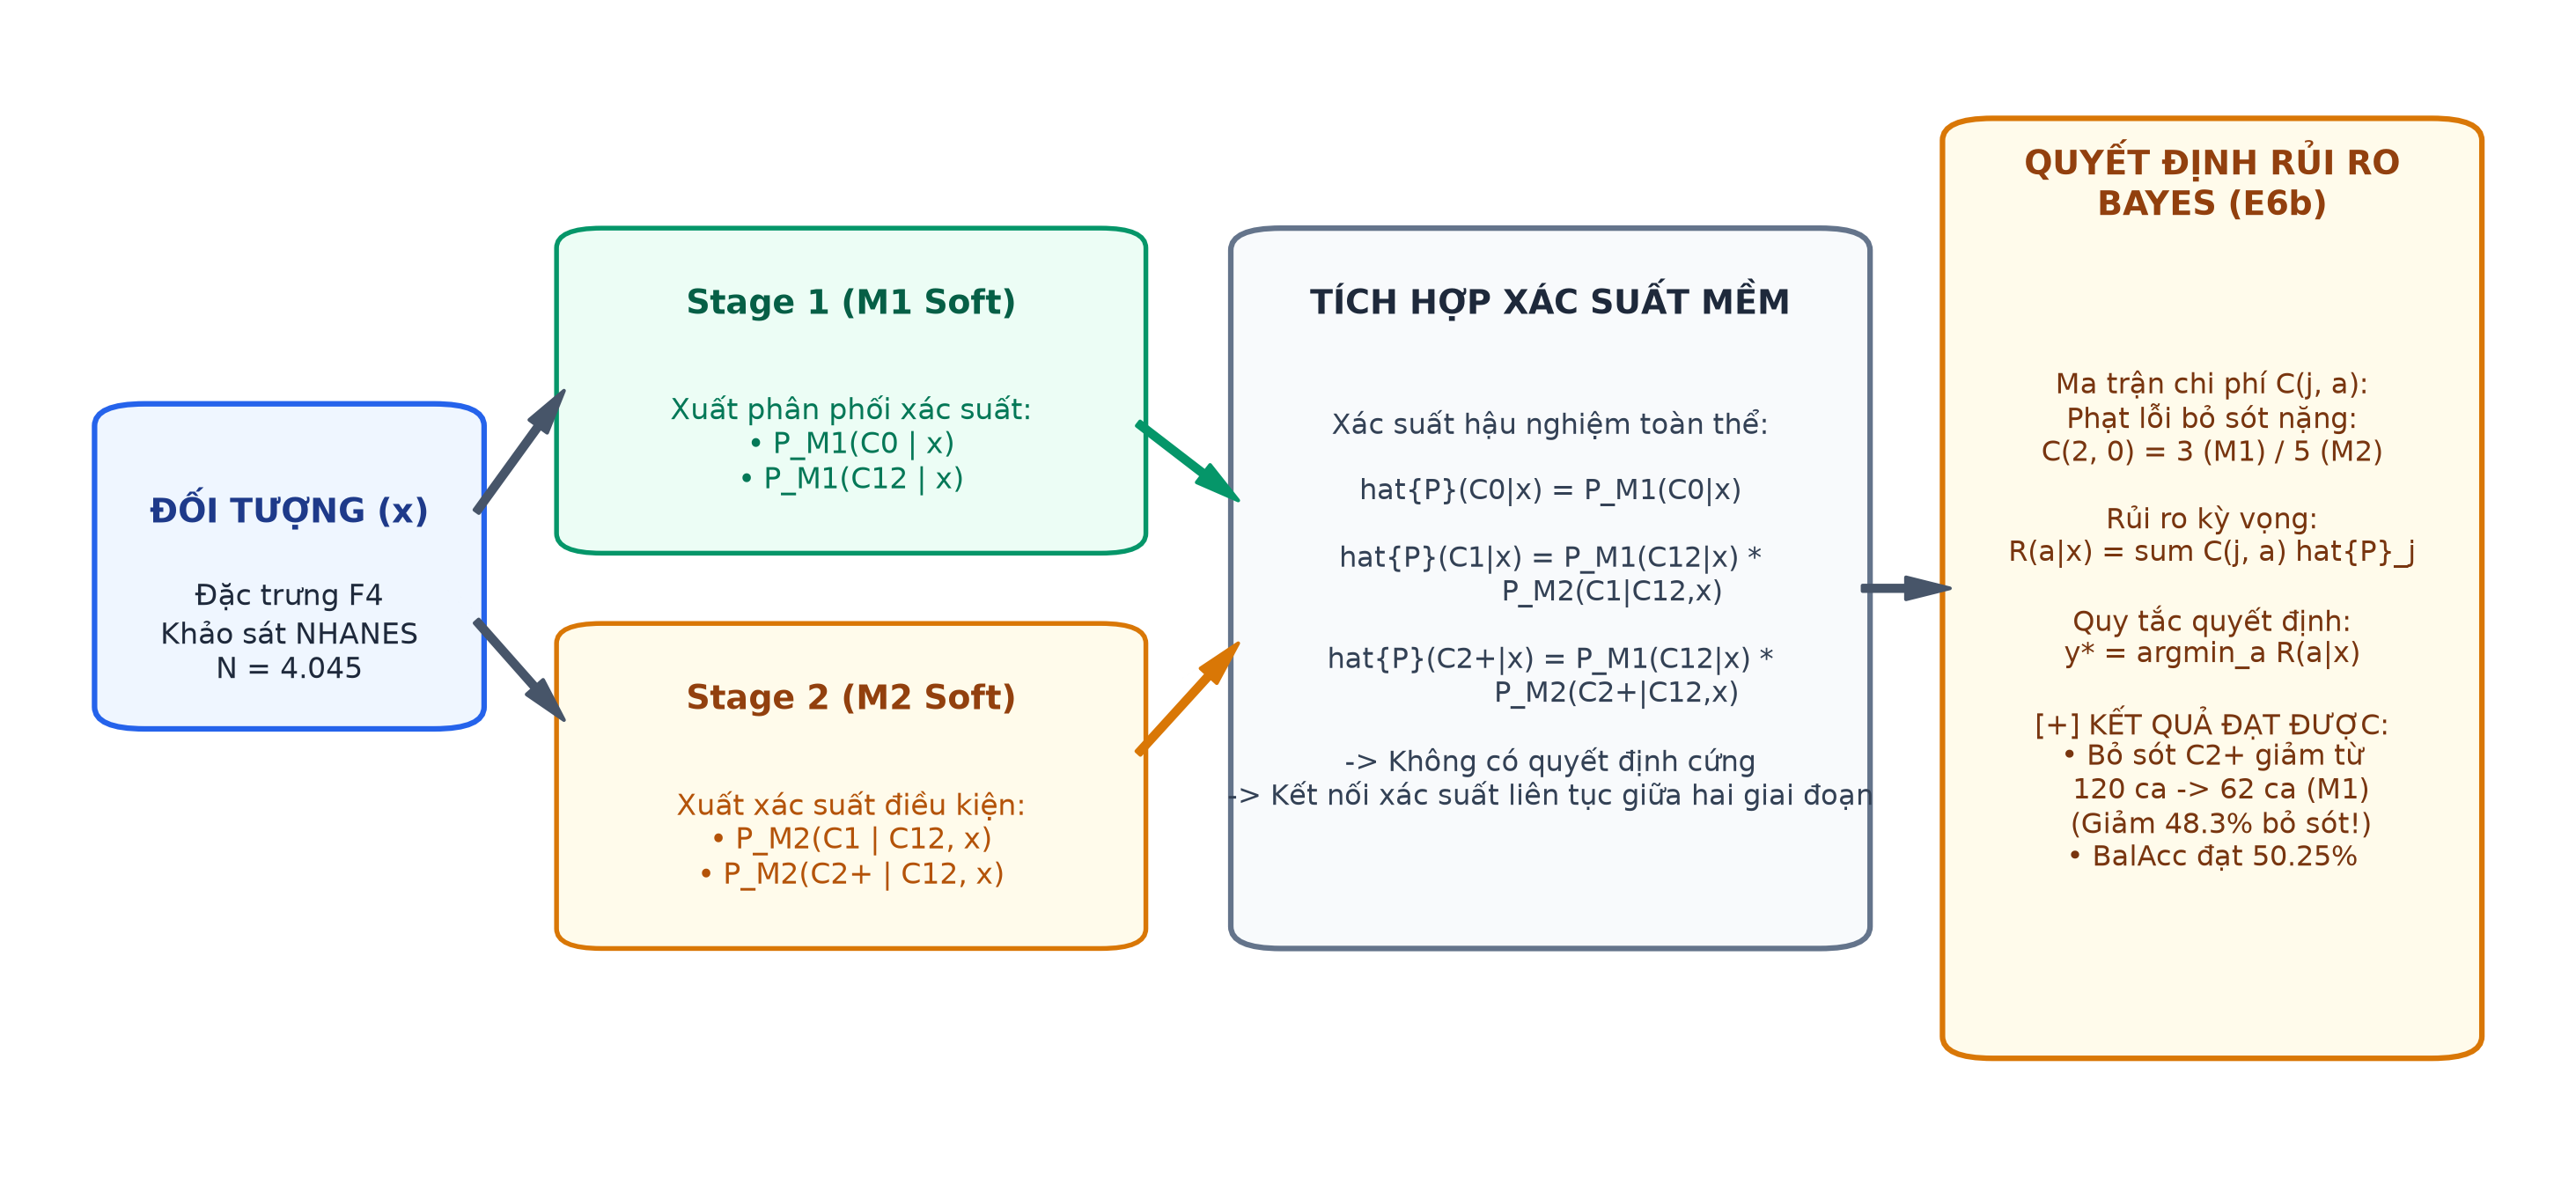
\includegraphics[width=\textwidth]{figures/fig3_5_soft_cost_sensitive.png}
\label{fig:soft-cost-architecture}
\end{figure}
\FloatBarrier

Phân phối xác suất hậu nghiệm kết hợp $\hat{\mathbf{p}} = [\hat{P}(C_0), \hat{P}(C_1), \hat{P}(C_2^+)]^T$ được tính theo công thức xác suất toàn phần:
\begin{align}
    \hat{P}(C_0 \mid \mathbf{x}) &= P_{M_1}(C_0 \mid \mathbf{x}) \\
    \hat{P}(C_1 \mid \mathbf{x}) &= P_{M_1}(C_{12} \mid \mathbf{x}) \cdot P_{M_2}(C_1 \mid C_{12}, \mathbf{x}) \\
    \hat{P}(C_2^+ \mid \mathbf{x}) &= P_{M_1}(C_{12} \mid \mathbf{x}) \cdot P_{M_2}(C_2^+ \mid C_{12}, \mathbf{x})
\end{align}

Từ phân phối xác suất hậu nghiệm mềm, hai cơ chế ra quyết định được áp dụng:
\begin{enumerate}
    \item \textbf{Cơ chế Argmax ($E_4, E_5$):} Chọn nhãn có xác suất lớn nhất $\hat{y} = \arg\max_k \hat{P}(C_k \mid \mathbf{x})$. Cấu hình $E_4$ sử dụng RF--RF; $E_5$ sử dụng RF--LR.
    \item \textbf{Cơ chế tối thiểu hóa rủi ro Bayes ($E_{6a}, E_{6b}$):} Đưa ma trận chi phí bất đối xứng $\mathbf{C} \in \mathbb{R}^{3 \times 3}$ vào hàm quyết định:
    \begin{equation}
        R(j \mid \mathbf{x}) = \sum_{i=0}^2 \hat{P}(C_i \mid \mathbf{x}) \cdot \mathbf{C}(i, j)
    \end{equation}
    \begin{equation}
        \hat{y}^* = \arg\min_{j \in \{0, 1, 2\}} R(j \mid \mathbf{x})
    \end{equation}
    trong đó $\mathbf{C}(i, j)$ là chi phí phạt khi nhãn thực tế là $C_i$ nhưng mô hình dự đoán là $C_j$. Nghiên cứu khảo sát 4 ma trận chi phí từ $M_0$ (chi phí đồng nhất) đến $M_3$ (phạt nặng nhất sai số bỏ sót ca nặng $\mathbf{C}(2, 0) = 8.0$). Ma trận được sử dụng chính trong báo cáo là $M_1$ ($\mathbf{C}(2, 0) = 3.0$). Chi tiết ma trận chi phí được trình bày tại Phụ lục \ref{app:cost-matrices}.
\end{enumerate}

\subsection{Mô hình phân loại thứ bậc ($E_7$)}
\label{subsec:e7-ordinal}

Do các mức độ triệu chứng PHQ-9 có tính chất thứ bậc ($C_0 < C_1 < C_2^+$), nhóm mô hình $E_7$ khai thác trực tiếp mối quan hệ trật tự này (Hình \ref{fig:ordinal-architecture}):

\begin{figure}[htbp]{Nguyên lý mô hình hóa thứ bậc: (a) Ordinal Logistic Regression và (b) Phân loại nhị phân tích lũy}
\centering
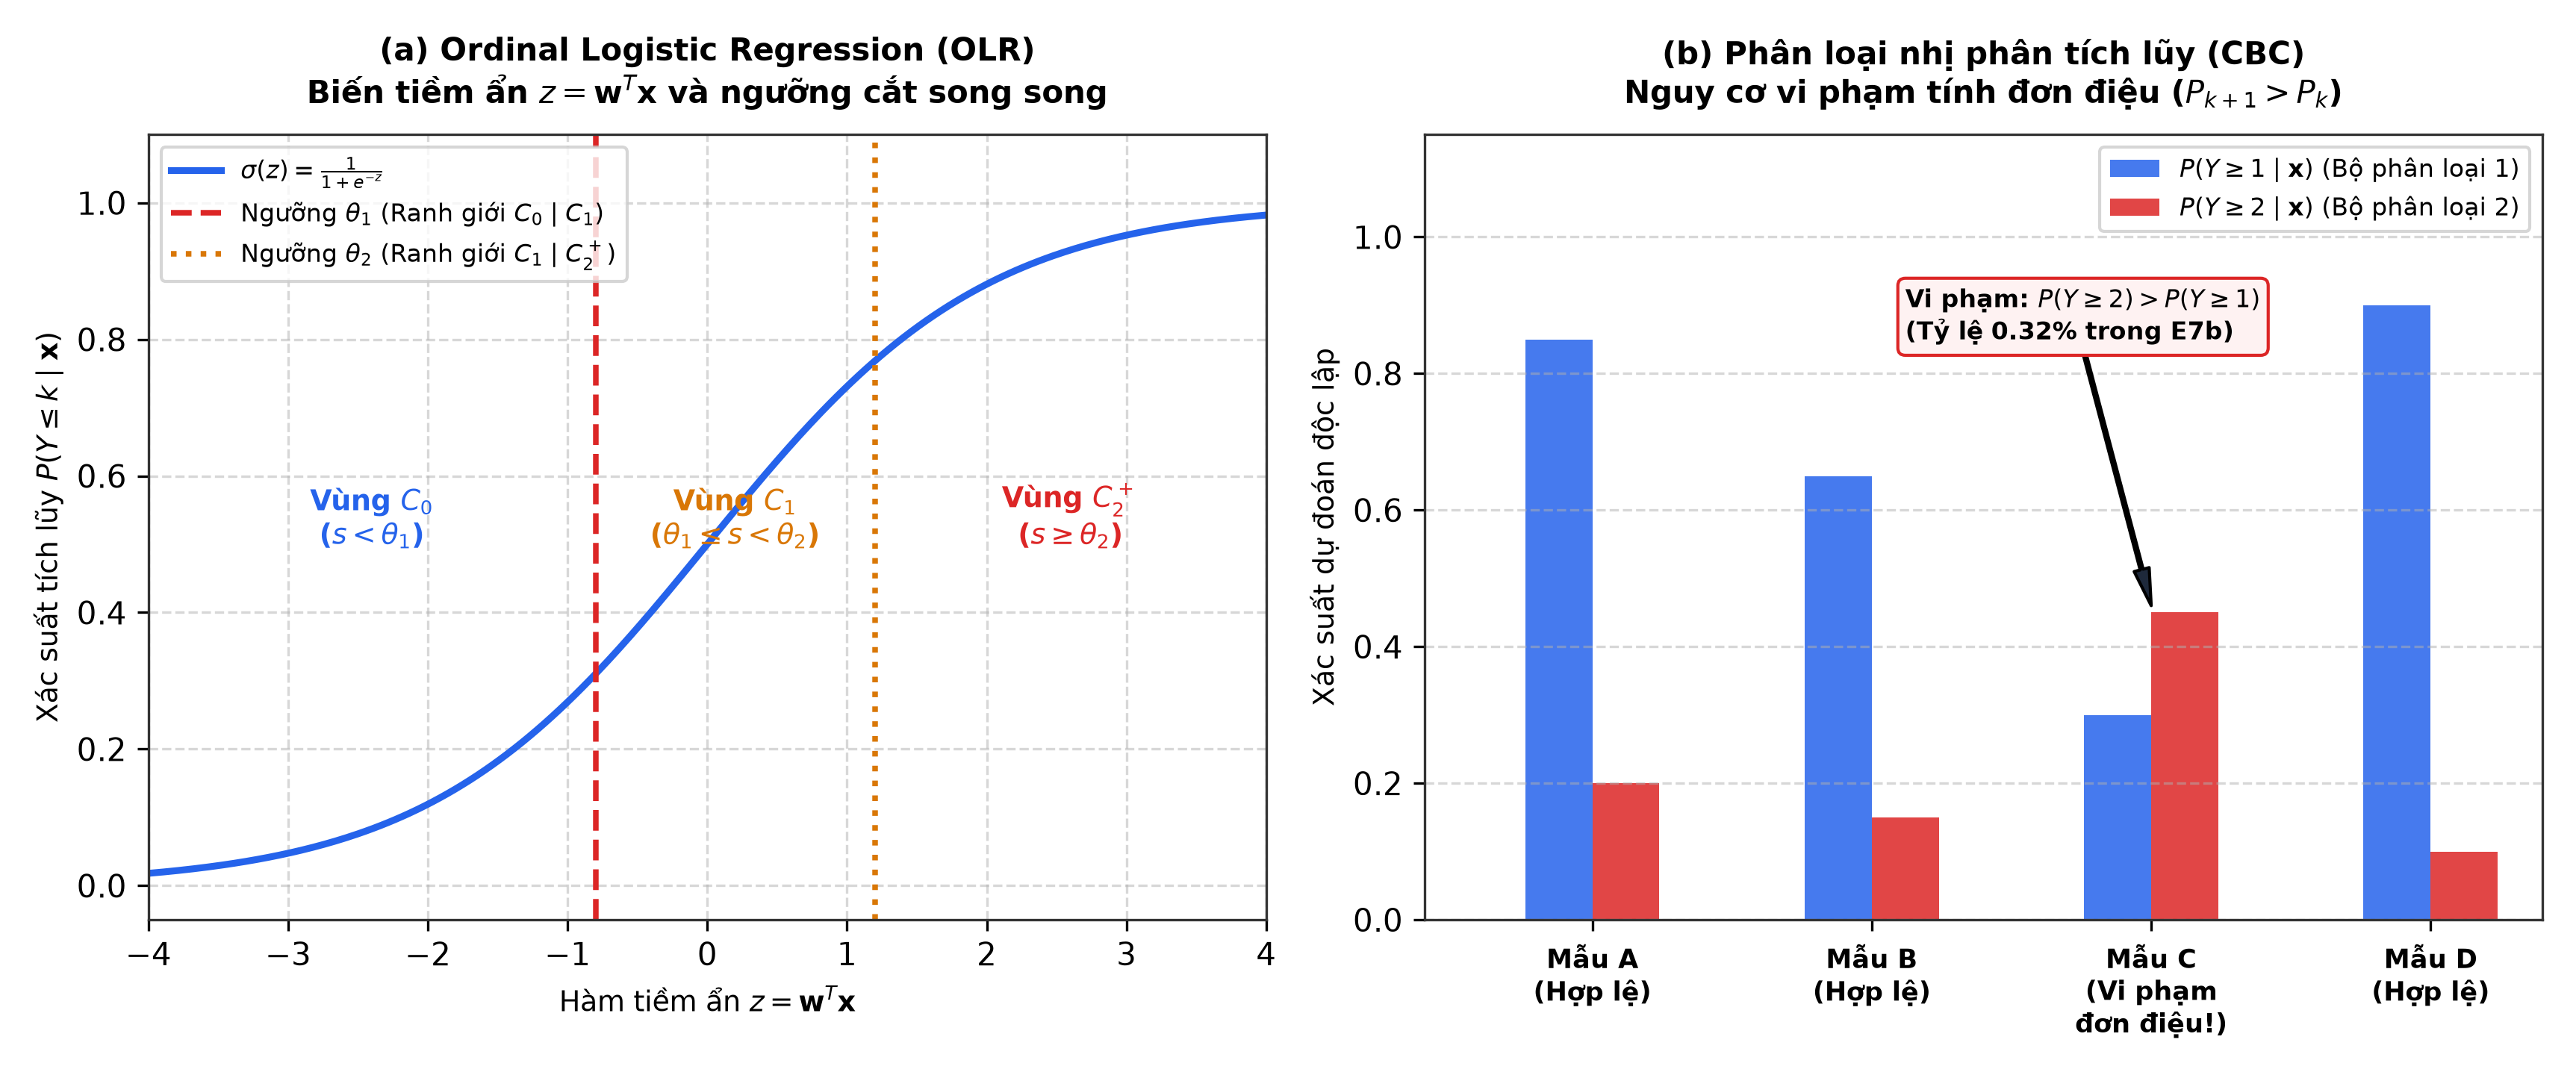
\includegraphics[width=\textwidth]{figures/fig3_6_ordinal_classification.png}
\label{fig:ordinal-architecture}
\end{figure}
\FloatBarrier

Nhóm thực nghiệm $E_7$ gồm hai hướng tiếp cận:
\begin{enumerate}
    \item \textbf{Ordinal Logistic Regression ($E_{7a}$ -- OLR):} 
    Mô hình giả định biến tiềm ẩn $z = \mathbf{w}^T \mathbf{x}$ cùng hai ngưỡng cắt $\theta_1 < \theta_2$. Xác suất tích lũy được mô hình hóa qua hàm phân phối Logistic:
    \begin{equation}
        P(Y \le k \mid \mathbf{x}) = \sigma(\theta_{k+1} - \mathbf{w}^T \mathbf{x}) = \frac{1}{1 + e^{-(\theta_{k+1} - \mathbf{w}^T \mathbf{x})}}
    \end{equation}
    Nghiên cứu khảo sát hai phiên bản: $E_{7a}$ Unweighted và $E_{7a}$ Balanced (gán trọng số nghịch đảo tần số lớp).
    \item \textbf{Phân loại nhị phân tích lũy ($E_{7b}$ -- Cumulative Binary Classification):} 
    Huấn luyện hai bộ phân loại nhị phân độc lập $h_1(\mathbf{x})$ cho bài toán $Y \ge 1$ và $h_2(\mathbf{x})$ cho bài toán $Y \ge 2$ bằng Random Forest. Xác suất từng lớp được suy luận bằng hiệu số tích lũy: $P(Y=0) = 1 - P(Y \ge 1)$, $P(Y=1) = P(Y \ge 1) - P(Y \ge 2)$, $P(Y=2) = P(Y \ge 2)$. Nếu xảy ra vi phạm đơn điệu $P(Y \ge 2) > P(Y \ge 1)$, giải thuật hiệu chỉnh ngưỡng cắt (isotonic clipping) được kích hoạt.
\end{enumerate}

\section{Thiết kế giao thức kiểm thử thực nghiệm}
\label{sec:giao-thuc-kiem-thu}

DepSev-ML áp dụng hai tầng giao thức kiểm định độc lập được minh họa trong Hình \ref{fig:evaluation-protocol}.

\begin{figure}[htbp]{Hai tầng giao thức kiểm thử: Nested 5-Fold Stratified CV và Temporal Validation}
\centering
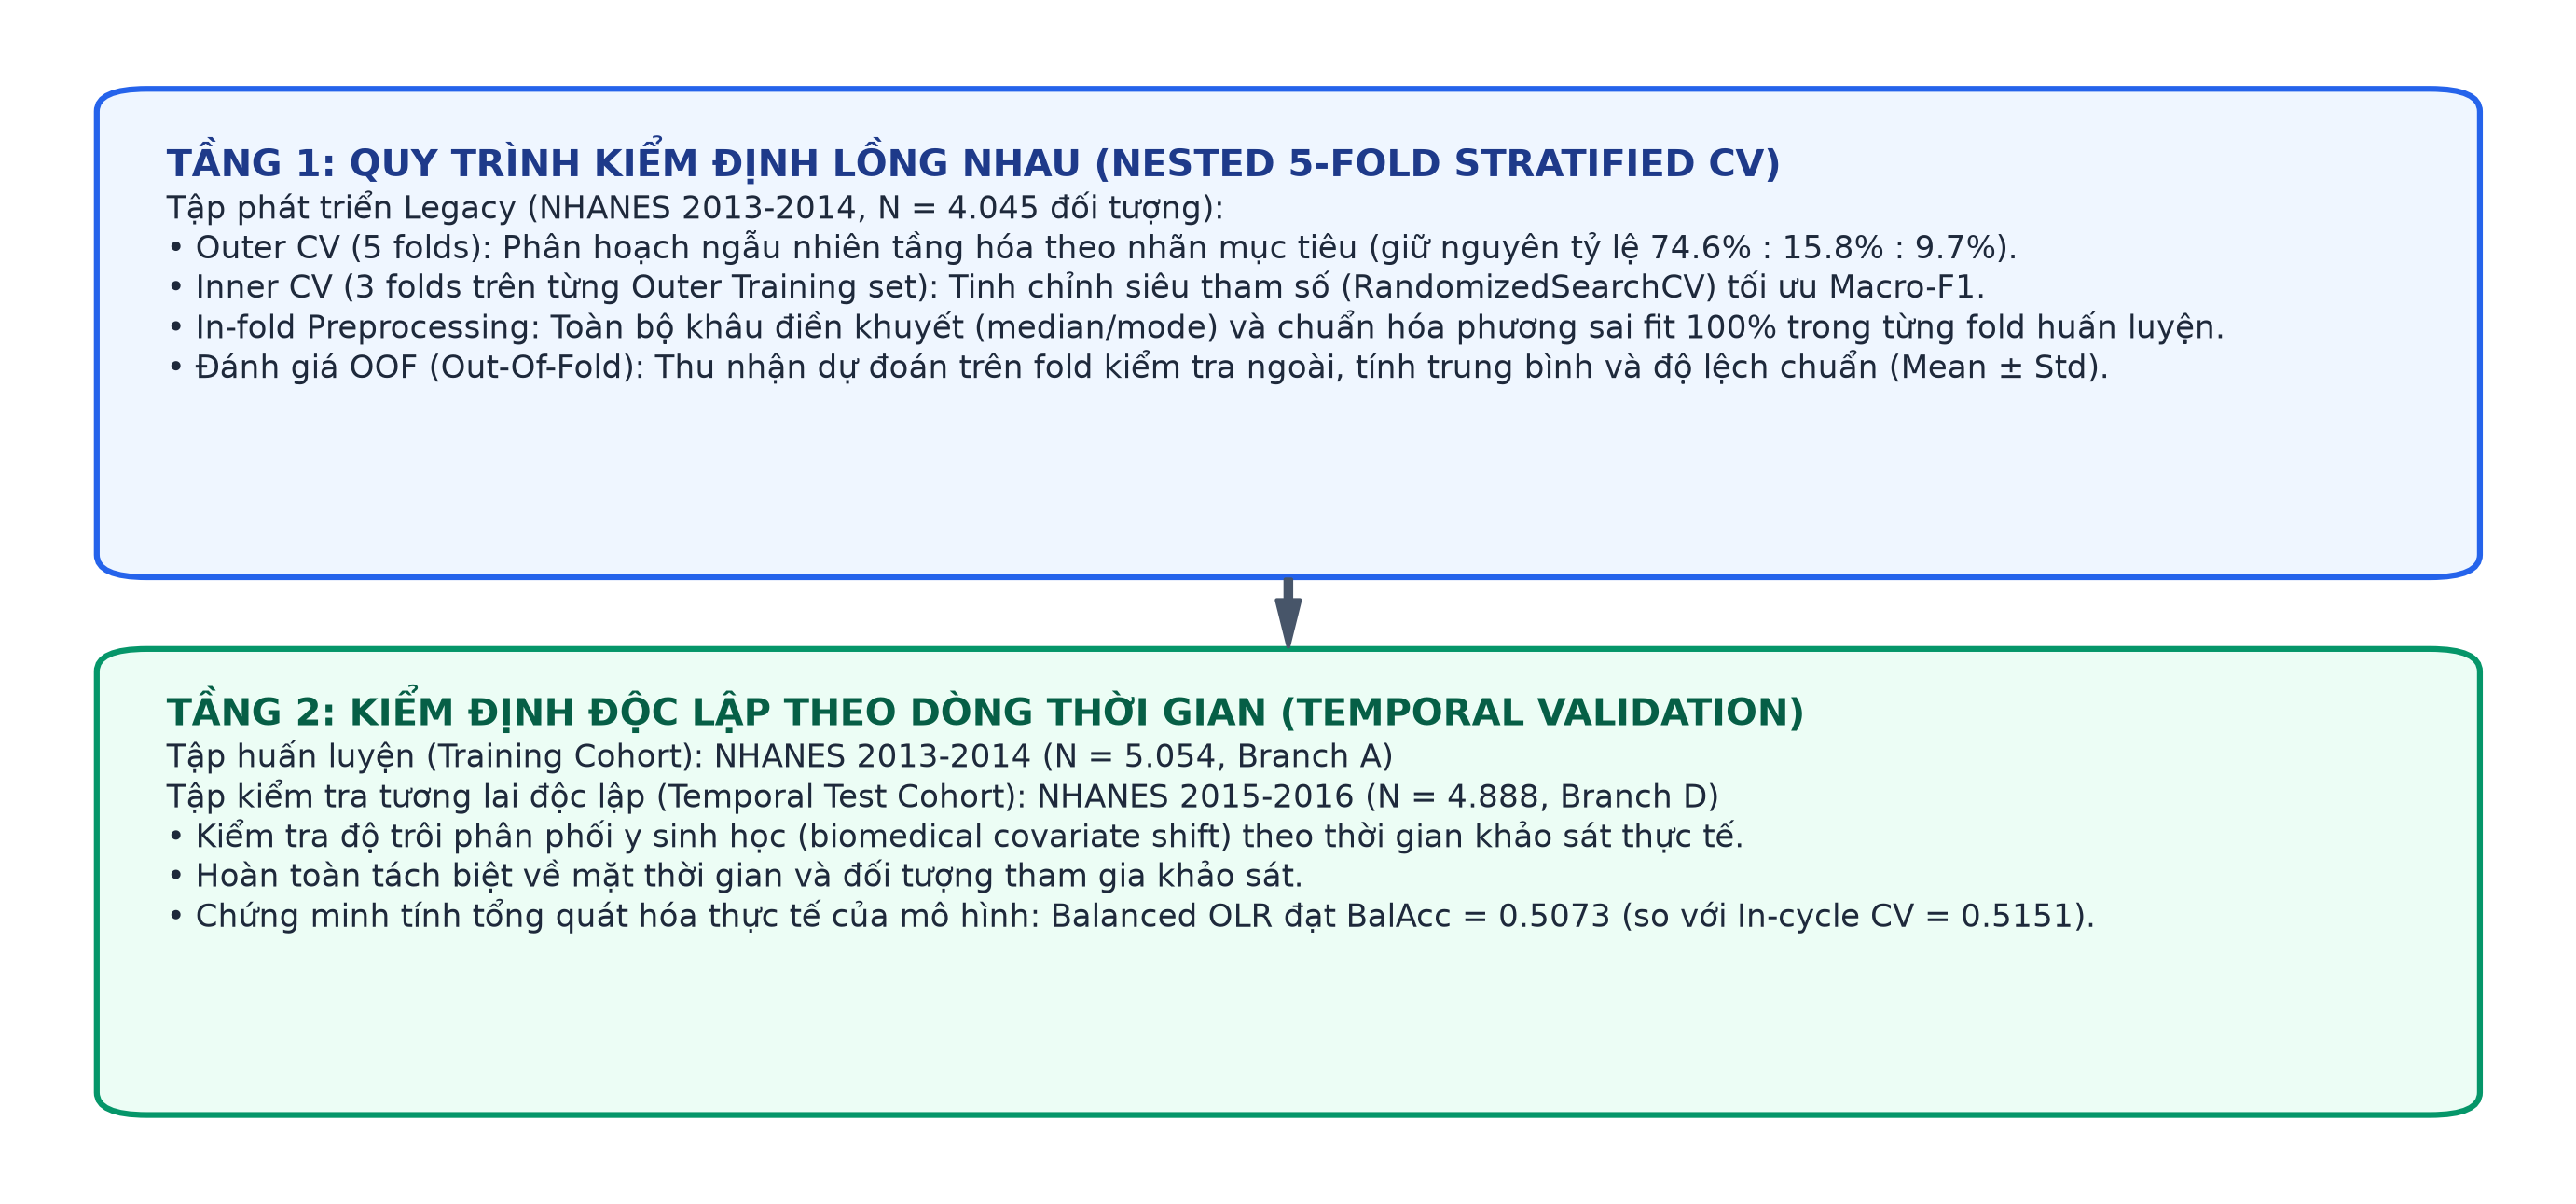
\includegraphics[width=\textwidth]{figures/fig3_7_evaluation_protocol.png}
\label{fig:evaluation-protocol}
\end{figure}
\FloatBarrier

\subsection{Quy trình kiểm định chéo lồng nhau (Nested 5-Fold Stratified CV)}
\label{subsec:nested-cv-protocol}

Trên tập dữ liệu phát triển Legacy ($N = 4.045$), quy trình kiểm định chéo lồng nhau được thực hiện:
\begin{itemize}
    \item \textbf{Outer CV (5 folds):} Phân chia dữ liệu thành 5 phần có bảo toàn tỷ lệ lớp (Stratified Split). Tại mỗi vòng lặp, 4 fold được dùng để huấn luyện và 1 fold dùng để đánh giá ngoài mẫu (Out-Of-Fold -- OOF).
    \item \textbf{Inner CV (3 folds trên từng Outer Training set):} Thực hiện \texttt{RandomizedSearchCV} với 12 cấu hình siêu tham số ngẫu nhiên trên độ đo Macro-F1 để tìm kiếm siêu tham số mà không sử dụng dữ liệu kiểm tra của Outer fold.
    \item Kết quả báo cáo là giá trị trung bình kèm độ lệch chuẩn ($\text{Mean} \pm \text{SD}$) trên 5 outer folds.
\end{itemize}

\subsection{Giao thức kiểm định ngoại suy theo dòng thời gian (Temporal Validation)}
\label{subsec:temporal-protocol}

Nhằm kiểm tra tính ổn định của mô hình trước hiện tượng dịch chuyển phân phối theo thời gian (covariate shift), nghiên cứu thiết lập giao thức kiểm định ngoại suy (Branch D): Tập huấn luyện gồm dữ liệu gộp hai chu kỳ NHANES 2011--2012 và 2013--2014 ($N = 9.693$); Tập kiểm tra độc lập gồm toàn bộ chu kỳ tiếp theo NHANES 2015--2016 ($N = 4.888$), áp dụng trên không gian 31 đặc trưng hài hòa hóa ($F_{4\_\text{common31}}$). Hai tập dữ liệu tách biệt về mặt thời gian khảo sát và không có đối tượng nào trùng lặp.

\section{Hệ thống độ đo đánh giá đa chiều}
\label{sec:he-thong-do-do}

Nghiên cứu sử dụng hệ thống chỉ số đánh giá gồm:
\begin{enumerate}
    \item \textbf{Macro-F1:} Trung bình cộng F1-score của toàn bộ các lớp, phản ánh khả năng nhận diện cân bằng giữa các lớp.
    \item \textbf{Balanced Accuracy (BalAcc):} Trung bình cộng của Recall từng lớp $\text{BalAcc} = \frac{1}{K}\sum_k \text{Recall}_k$.
    \item \textbf{Class MAE (Sai số tuyệt đối theo lớp):} Đo khoảng cách trung bình giữa mức độ dự đoán và mức độ thực tế: $\text{Class MAE} = \frac{1}{N} \sum_{i=1}^N |y_i - \hat{y}_i|$.
    \item \textbf{Quadratic Weighted Kappa (QWK):} Đo lường mức độ đồng thuận thứ bậc có tính đến mức phạt khoảng cách \cite{cohen1968weighted}.
    \item \textbf{Đánh giá mức độ bỏ sót ca nặng:} Số lượng ca nặng bị bỏ sót thành bình thường ($C_2^+ \to C_0$) và số ca báo động nhầm ($C_0 \to C_2^+$).
\end{enumerate}

\section{Tóm tắt chương}
\label{sec:tom-tat-chuong-3}

Chương 3 đã trình bày phương pháp luận của đề tài: từ quy trình tiền xử lý in-fold kiểm soát rò rỉ dữ liệu, 4 không gian đặc trưng lũy tiến ($F_1 \to F_4$), các thiết kế mô hình thực nghiệm ($E_0 \to E_7$), đến hai tầng giao thức kiểm định (Nested CV và Temporal Validation). Toàn bộ kết quả thực nghiệm thu được sẽ được phân tích chi tiết trong Chương \ref{ch:thuc-nghiem}.
